% !TeX root = ../main.tex

\chapter{医学文本生成任务推断阶段的隐私保护研究}

\section{引言}

为防止攻击者在推断阶段试图通过模型反演攻击来恢复训练隐私数据,同时保持语言模型的表现效果,本章基于差分隐私算法提出两种方法来缓解语言模型的记忆问题,从而保护隐私数据。首先,本章将介绍系统模型与设计目标,引入本章的保护对象与攻击者的行为。其次,介绍选择差分隐私的定义,并针对训练与推断阶段分别设计了隐私优化器与解码算法,作为两种提供选择差分隐私的方式。随后,对前述设计的隐私优化器与解码算法进行隐私性分析,以证明其满足差分隐私的定义。最后,通过设计实验说明这两种保护方式的优势。

\section{系统模型与设计目标}

\subsection{系统模型}

如图\ref{Chap5_Attatck_Model}所示,在这种场景下,拥有隐私医学文本数据集的数据持有者通过一种训练策略得到一个针对该领域医学文本的语言模型,其通过公开推断查询的接口来提供查询服务。正常的诚实使用者将输入传给模型持有者,模型持有者通过语言模型执行推断,并将语言模型的输出返回给使用者。而调用查询接口的使用者可能会定制攻击输入前缀并通过执行多次推断服务来尝试恢复模型的隐私数据。

本节研究持有隐私数据集的数据持有者如何保障在执行推断阶段时,训练好的语言模型不会由于“记忆性”导致泄露出训练的隐私内容,即使用何种训练策略才能让模型主要关注于文本构成以及生成逻辑,而不是“记住”具体的隐私信息。因此,本节考虑两个实体,第一个是拥有隐私医学文本数据集的数据持有者,第二个是调用查询接口的使用者。



%另一方是通过模型持有者接口进行查询的使用者。多个数据持有者希望通过多个计算方提供的计算服务来协同训练模型,计算方在计算服务结束后将训练好的模型分发给各个数据持有者。

%如图\ref{Chap4_System_Info}所示,其中①表示多个数据持有者通过秘密共享算法将数据拆分成两个秘密份额分发给服务器$p_0$与服务器$p_1$。②表示在服务器$p_2$提供的相应MPC计算随机数的辅助下,服务器$p_0$与服务器$p_1$运行MPC协议来执行模型的训练过程。③表示训练结束后,服务器$p_0$与服务器$p_1$将各自的模型参数份额返还给各数据持有者。在这种场景下,我们假设有两类实体,一方是多个拥有医疗隐私数据的数据持有者,另一方是提供计算服务的三个计算方。多个数据持有者希望通过多个计算方提供的计算服务来协同训练模型,计算方在计算服务结束后将训练好的模型分发给各个数据持有者。其中作为提供计算服务的三个计算方$p_0$、$p_1$与$p_2$均具有Intel SGX,且$p_0$与$p_1$具有高性能计算GPU或者TPU(后文均以GPU指代)。

\begin{figure}[h]
	\centering
	%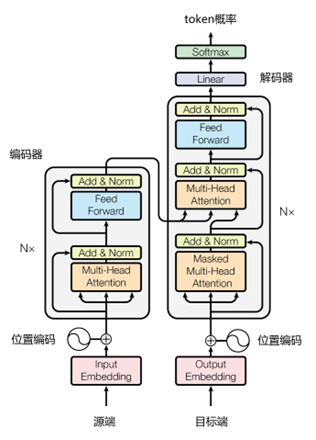
\includegraphics[width=1\textwidth]{figures/Transformer_Structure.png}sep_exeEncalveE
	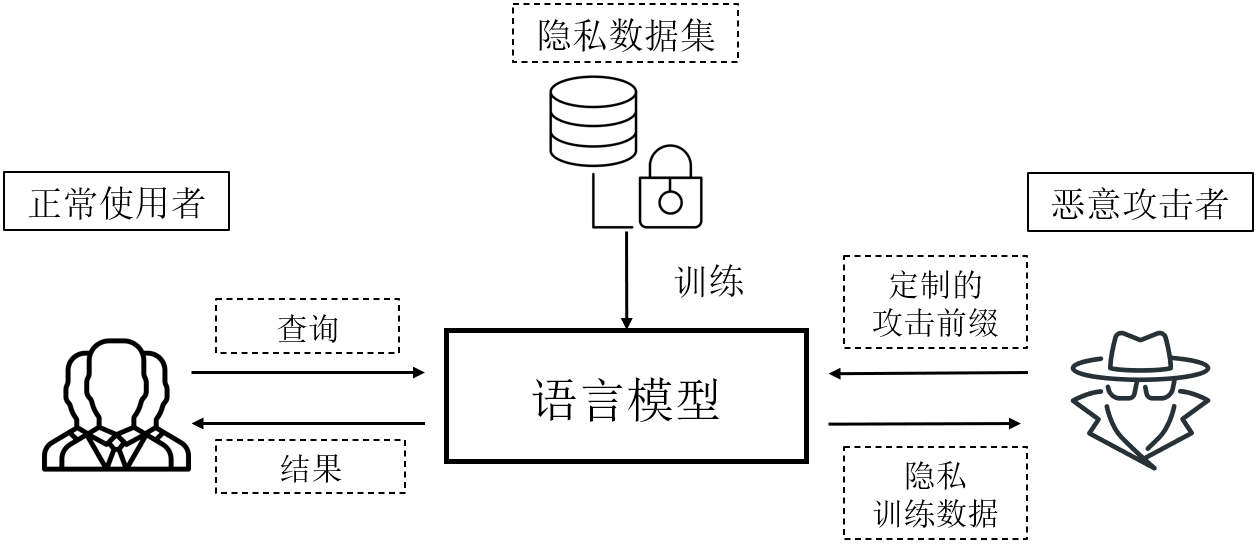
\includegraphics[width=0.7\linewidth]{figures/Chap5_Attack_Model.png}
	\caption{公布模型查询接口的风险}
	\label{Chap5_Attatck_Model}
\end{figure}

\subsection{威胁模型与设计目标}

(1)威胁模型

本节对该场景下拥有隐私医学文本数据集的数据持有者的安全假设是诚实的,即它会使用真实的医学隐私训练语料通过特定的训练方式来训练模型,也称为模型持有者(后文提到的数据持有者与模型持有者在本章中都是相同的)。对于调用查询接口的使用者,本章假设其是恶意的,它可以通过定制任何攻击前缀来从模型持有者的模型中推断训练数据集的隐私信息。

(2)设计目标

\begin{itemize}
	\item [a)]
	训练阶段引入差分隐私。数据持有者通过一个隐私保护的训练算法在隐私数据上进行模型训练,推断阶段直接输出推断结果。
	\item [b)]
	推断阶段引入差分隐私。数据持有者直接使用隐私数据进行训练,推断阶段使用一个隐私保护的推断算法输出推断结果。
\end{itemize}

%\section{选择差分隐私算法}

\section{基于差分隐私算法的推断结果隐私保护方案}

\subsection{选择差分隐私定义}

参考\ref{NLP_Def}节的介绍,考虑一个由词表$V$中的多个tokens组成的文本序列,即$x=(x_1,\dots,x_n)$,其中$x_i$为第$i$个token。语言建模的目标是,通过应用链式法则$Pr(x)=∏_{i=1}^n Pr(x_i |x_{<i})$构建分布的生成模型$Pr(x)$。当用参数$\theta$评估神经网络$f$时,本节让$f_\theta(x_i|x_{<i})$表示token $x_i$的概率。通过训练最小化负对数似然函数$L(θ) = -log ∏_{i=1}^n f_θ (x_i|x_{<i})$,来使得模型最大化训练集$W$中数据的概率。
$$Pr(x)=∏_{i=1}^n p(x_i|x_{<i})$$
$$L(θ)=-∑_{t=1}^{|D|} ∑_{i=1}^{n_t} log p_\theta (x_i^t |x_{<i}^t)$$

由\ref{eps-delta-dp}中DP的定义,若将DP直接部署在医学文本生成任务上,其对所有内容进行保护,即将所有记录视为敏感的。相关工作研究了在NLP领域使用DP的一些变体,如个性化DP\cite{DP_Personal}和onesided DP\cite{onesideDP}。然而,现有的隐私概念不允许给定记录中的不同属性具有不同的隐私级别,特别是对于隐私属性极为稀疏的NLP任务。因此,我们提出了一种新的隐私概念——选择差异隐私,即使用策略函数区分一个数据样本内部的私有和非私有属性,并保护一个数据样本的私有部分。


\begin{definition}{(策略函数)}
	策略函数$F: τ\rightarrow\{0,1\}^{n_r}$表示一个记录$r∈τ$的哪些属性是敏感的$(F(r)_i=0)$或不敏感的$(F(r)_i=1)$,其中$n_r$是$r$中的属性数量。其中,$n_r$依赖于记录,而不是一个固定的数。
	\label{metric_func}
\end{definition}

用户可以自由定义策略函数来编码具体的隐私规定,并根据具体应用保护任何敏感属性。受保护的敏感属性类型是无限的,可以是实体(如姓名、电子邮件等)、上下文(如健康相关信息、说话风格等),等等。例如,用户可以设计一个保守的政策功能,在必要时保护选定的完整句子。策略函数的形式也是无限的,可以是神经网络、正则表达式等。

在语言建模的情况下,每个记录是一个文本序列$x$,每个属性是$x$中的一个token $x_i$, $F(x)$是一个位向量,表示哪些标记包含私有信息。我们在新的隐私概念下定义如下所示的相邻数据集。

\begin{definition}{(F-Neighbors)}
	$D, D'$是两个数据集,$F$是一个策略函数。当且仅当$∃r∈D$使得$F(r)$包含至少一个私有属性,$∃r'∈D'$ 使得$F(r)$和$F(r')$至少有一个私有属性不同,且$D'=D\\{ r}∪{ r'}$时,我们称$D'$是$D$的相邻数据集。我们简记为 $D'∈N_F (D)$。
	\label{F_Neighbour}
\end{definition}

在这个定义下,包含“我的ID是123”的数据集和包含“我的ID是456”的数据集是相邻的。但带有“Hello there”的数据集和带有“Hi there”的数据集不是邻居,因为它们不包含隐私信息。

\begin{definition}{(选择差分隐私\cite{selectivedp})}
给定一个策略函数$F$。对于$∀D, D'\in N_F (D)$以及$∀T⊆R$,如果$Pr[M(D)\subset T]\leq e^\epsilon Pr[M(D')\subset T]+\delta$,我们称随机算法$M:D\rightarrow R$满足$(F,\epsilon,\delta)$-Selective DP。
\label{SDP}
\end{definition}

本质上,选择性差分隐私也提供了类似于规范DP的不可区分性,但只针对记录中的敏感属性。只要保留敏感属性的隐私,选择性差分隐私并不约束非敏感属性的信息泄露。因此,选择性差分隐私在最坏的情况下(即攻击者可能知道除目标敏感属性之外的所有信息)保护敏感属性的隐私。

\subsection{针对训练阶段的选择差分隐私优化器}


%本节介绍针对训练阶段的选择差分隐私优化器。使用选择差分隐私机制的相关工作\cite{selectivedp}仅在RNN式的语言模型上实施。RNN式的模型按照token出现的顺序从前往后滑动处理,这种情况下隐私tokens与非隐私token分开处理较容易,而由于基于Transformer结构的模型所有tokens时并行处理的,因此无法直接将研究工作\cite{selectivedp}中的RNN式的处理方法用在基于Transformer的模型上。下面引入本节针对训练阶段的选择差分隐私优化器的介绍。

本节介绍针对训练阶段的选择性差分隐私优化器。虽然使用选择性差分隐私机制的相关工作\cite{selectivedp}已在RNN式的语言模型上实施,但RNN式的模型按照token出现的顺序从前往后滑动处理,这种情况下较容易分开处理隐私tokens与非隐私tokens。而基于Transformer结构的模型中,所有tokens是并行处理的,因此无法直接将研究工作\cite{selectivedp}中的RNN式处理方法应用于基于Transformer的模型。接下来,本部分将详细介绍针对训练阶段的选择性差分隐私优化器。

%如图\ref{SDP_Optim}和算法\ref{Algrithm_SDP_Optim}所示,用于训练基于Transformer(下文表示为Model)的语言模型,实现S-DP。其基本思路是先用策略函数确定私有属性,然后确定哪些模型变量与私有属性相关,最后对非私有变量应用常规Optimizer,对私有变量应用DP-Optimizer,如图\ref{SDP_Optim}所示。

如图\ref{SDP_Optim}和算法\ref{Algrithm_SDP_Optim}所示,该优化器用于训练基于Transformer(以下简称为Model)的语言模型,实现选择差分隐私。其基本思路首先使用策略函数确定私有属性,然后确定哪些模型变量与私有属性相关,最后对非私有变量应用常规Optimizer,对私有变量应用DP-Optimizer(如图\ref{SDP_Optim}所示)。

这里需要首先确定与私有tokens相关的变量。Model使用一个隐藏状态$h_i$对上下文进行编码,输出在词表$V$上的一个分布$p_i$。如果$x_i$是私有的,那么$h_i$、$p_i$和$L_i$都是私有的。

%$$h_i=Model(h_{i-1},x_i)$$
%$$p_i=p_\theta(V|x_{<i})=Softmax(g(h_i))$$
%$$L_i=-log p_\theta(x_{i+1}|x_{<i+1})$$


\begin{figure}[h]
	\centering
	%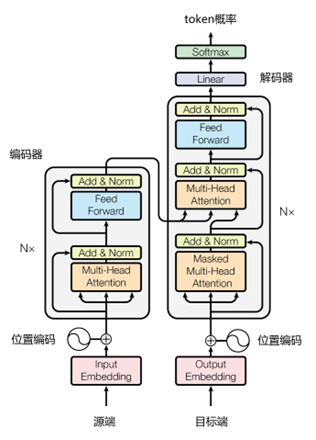
\includegraphics[width=1\textwidth]{figures/Transformer_Structure.png}
	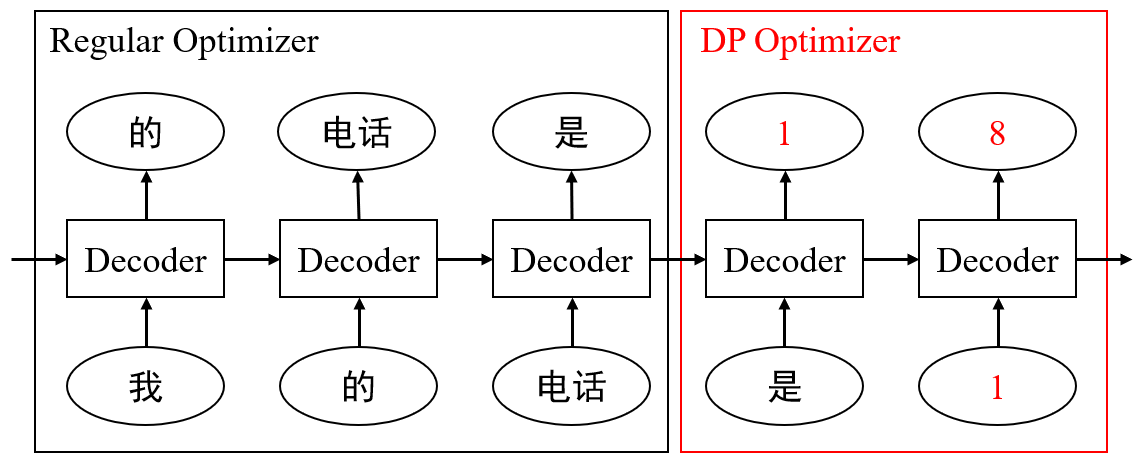
\includegraphics[width=0.7\linewidth]{figures/SDP_Optim.png}
	\caption{差分隐私训练优化器}
	\label{SDP_Optim}
\end{figure}


%\begin{algorithm}[H]
%	% \renewcommand{\thealgocf}{}     %<---细节与重点
%	\SetAlgoLined
%	\KwIn{$N$个样本的数据集$D$,策略函数$F$,隐私矩阵$P=F(D)$,最大序列长度$K$,损失函数$L(\theta)$,超参数:学习率$\eta$、噪声指数$\sigma$、梯度裁剪上界$C$、组大小$L$,模型参数$\rm Model$}
%	
%	\KwOut{模型经过一轮训练更新后的参数$\rm Model$}
%	
%	\For{$t = 1, 2, \dots$}{
%		
%		对数据集$D$中长度不超过最大序列长度$K$的样本进行采样,组成$\frac{L}{N}$个batch $B$
%		
%		使用隐私矩阵$P=F(D)$将$B$中的数据拆分成非隐私元组与隐私元组:$\{(B_{np, i}, B_{p, i})\}$
%		
%		初始化$h=0$
%		
%		\For{$i = 1, 2, \dots$}{
%			\# 1) 常规更新 Regular update
%			
%			$L, h = $$\rm Model$$(B_{np, i}, h)$
%			
%			$\theta \leftarrow \theta - \eta \nabla_\theta L(\theta)$
%			
%			\# 2) 隐私更新 Private update
%			
%			$L, h = $$\rm Model$$(B_{np, i}, h)$
%			
%			\# 计算样本梯度
%			
%			对于每一个$x_j\in B_{p, i}$,计算$g(x_j) \leftarrow \nabla_\theta L(\theta, x_j)$
%			
%			\# 梯度裁剪
%			
%			$g(x_j) \leftarrow g(x_j) / max(1, \frac{\Vert g \Vert_2}{C})$
%			
%			\# 加噪
%			
%			$g(x_j) \leftarrow \frac{1}{|B_{p, i}|} (\sum_j g(x_j) + \sigma C\cdot N(0, I))$
%			
%			\# 梯度下降
%			
%			$\theta \leftarrow \theta - \eta \nabla_\theta L(\theta)$
%			
%			\# 裁剪隐层表示
%			
%			$h(x_j) \leftarrow h(x_j) / max(1, \frac{\Vert h \Vert_2}{C})$
%			
%			\# 加噪
%			
%			$h(x_j) \leftarrow h(x_j) + \sigma C\cdot N(0, I)$
%			
%			
%			
%		}
%		
%	}
%	
%	\caption{Partial-DP-Optimizer}
%	\label{Algrithm_SDP_Optim}
%\end{algorithm}

\begin{algorithm}[H]
	% \renewcommand{\thealgocf}{}     %<---细节与重点
	\SetAlgoLined
	\SetKwInOut{Input}{输入}
	\SetKwInOut{Output}{输出}
	\Input{$N$个样本的数据集$D$,策略函数$F$,隐私矩阵$P=F(D)$,最大序列长度$K$,损失函数$L(\theta)$,超参数:学习率$\eta$、噪声指数$\sigma$、梯度裁剪上界$C$、批大小$B$,模型参数$\rm Model=\{Token\_Embedding, Encoder, Vocab\_Projection\}$}
	
	\Output{模型经过一轮训练更新后的参数$\rm Model$}
	
	\For{$j = 1, 2, \dots, B$}{
		
		%记Batch\_input[i]中第$j$个句子的内容Batch\_input[i][j]为Sen
		
		\For{$k = 1, 2, \dots, len(Sen)$}{
			记$\rm Batch\_input[i]$的第$j$个句子$\rm Batch\_input[i][j]$为$x$
			
			使用隐私矩阵$\rm P=F(input)$将$B$中的数据拆分成非隐私元组与隐私元组:$\rm \{(M_{np}, M_{p})\}$
			
			$\rm E = Token\_Embedding(x)$
			
			$\rm Out\_E = Encoder(E)$
			
			\For{$\rm x_k\in M_{p}$}{

				$Out\_E_{p}\leftarrow Out\_E_{p} / max(1, \frac{\Vert Out\_E \Vert_2}{C})$

				$Out\_E_{p} \leftarrow Out\_E_{p} + \sigma C\cdot N(0, I)$
			}

			$\rm Logits[j] = Vocab\_Projection(Out\_E[-1])$
			
		}
		
		\For{$k = 1, 2, \dots, len(Sen) - 1$}{			
			%$Loss[k] = L(Logits[k], x[k + 1])$
			\If{$\rm k\in M_{p}$}{
			%\For{$\rm k\in M_{p}$}
				$g(k) \leftarrow \nabla_\theta L(\theta, Logits[k], x[k + 1])$
				
				$g(k) \leftarrow g(k) / max(1, \frac{\Vert g \Vert_2}{C})$

				$g(k) \leftarrow \frac{1}{|M_{p}|} (\sum_j g(k) + \sigma C\cdot N(0, I))$

				$\theta \leftarrow \theta - \eta g(k)$		
			}
			\Else{$\theta \leftarrow \theta - \eta \nabla_\theta L(\theta)$	}		
		}
	}
	
	\caption{选择差分隐私优化器}
	\label{Algrithm_SDP_Optim}
\end{algorithm}

算法\ref{Algrithm_SDP_Optim}概述了DP-Optimizer中的步骤。给定一个数据集$D$,我们应用一个策略函数$F$来获得一个比特矩阵$P=F(D)$,表示哪些tokens是私有的。在每一步,我们取一个随机batch $B$,并使用$P$将$B$拆分成一个非私有和私有元组的序列${(B_{np,i},B_{p,i})}$;然后我们在$B_{p,i}$上应用Optimizer (常规更新),在$B_{p,i}$上应用DP-Optimizer (隐私更新),交替进行,以更新和保护隐私。注意,除了梯度中的噪声,如果隐藏状态$h_i$是私有的,我们还对其裁剪和添加噪声。原因是在LM中,如果$x_i$是私有的,$h_i$也包含私有信息(如上所示),并且直接传递给下一个常规更新步骤,无法被梯度中的噪声保护。所以在$h_i$中加入噪声来保护隐私信息是很重要的。由于DP-Optimizer对梯度增加了噪声,用于计算损失的$L$和$p_i$被梯度中的噪声保护。这样一来,所有的私有变量都得到了保护。


\subsection{针对推断阶段的选择差分隐私解码算法}


\begin{figure}[h]
	\centering
	%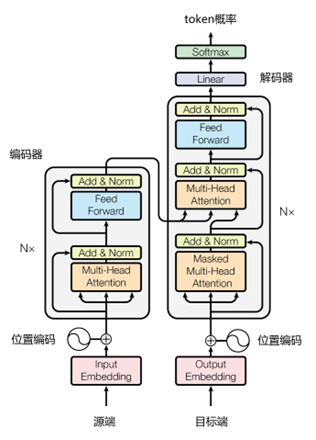
\includegraphics[width=1\textwidth]{figures/Transformer_Structure.png}
	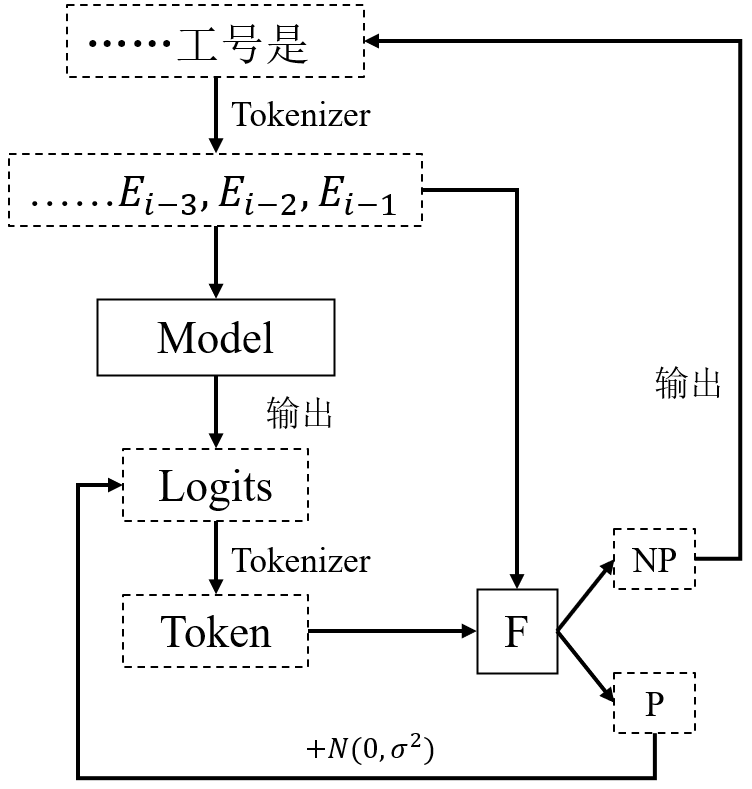
\includegraphics[width=0.5\linewidth]{figures/Chap5_PDP_Decode.png}
	\caption{差分隐私解码算法}
	\label{Chap5_PDP_Decode}
\end{figure}



\begin{algorithm}[H]
	% \renewcommand{\thealgocf}{}     %<---细节与重点
	\SetAlgoLined
	\SetKwInOut{Input}{输入}
	\SetKwInOut{Output}{输出}
	\Input{输入解码的前缀$P$,策略函数$F$,裁剪上界$C$、组大小$L$,模型$\rm Model$,词表$V$,分词器Tokenizer($\cdot$)}
	
	\Output{输入解码的前缀为Prefix时,模型的输出结果Output}
	
	\# 将当前生成结果记为CS,初始赋值为输入前缀
	
	CS = P
	
%	\# PS为策略函数输出的隐私分类,初始赋值为False,即认为所有输入前缀均非敏感
%	
%	PS = [False] * len(P)
	
	\# 模型输出预测下一个Token的Logits
	
	NT\_Logits = Model(CS)
	
	\# Logits确定最大概率的index,并由分词器解码成输出字符
	
	NT = Tokenizer.decode(argmax(Softmax(NT\_Logits)))
	
	\# 若输出<EOS>符号终止流程
	
	\While{NT != <EOS>}{
		
		\# 若已生成内容与当前预测的下一个Token在策略函数$F$下是隐私内容,则需要加噪处理
		
		\If{F(CS, NT) == True}{
			\# 对Logits进行裁剪
			NT\_Logits $\leftarrow$ NT\_Logits / max(1, $\frac{\Vert NT\_Logits \Vert_2}{C}$)
			
			\# 加噪
			
			NT\_Logits \leftarrow NT\_Logits + $\sigma C\cdot N(0, I)$
			
			\# 在加噪的Logists下重新生成Token
			
			NT = Tokenizer.decode(argmax(Softmax(NT\_Logits)))
		}
		
		\# 将新Token加入当前生成结果CS中
		
		CS = CS + NT
		
		\# 继续预测下一个Token的Logits
		
		NT\_Logits = Model(CS)
		
		\# 由分词器对index进行解码
		
		NT = Tokenizer.decode(argmax(Softmax(NT\_Logits)))
	}

	
	\caption{选择差分隐私解码算法}
	\label{Algrithm_SDP_Decoding}
\end{algorithm}

如图\ref{Chap5_PDP_Decode}与算法\ref{Algrithm_SDP_Decoding}概述了针对推断阶段的解码算法。由于该场景下训练阶段使用原始包含隐私内容的数据集进行训练,在推断阶段时,为保护隐私内容,需要对生成结果进行处理。具体来说,在生成输出的过程中,使用策略函数$F$对已生成的内容与当前模型输出的下一个Token进行判断,若属于隐私内容,则对Logits进行裁剪并加上由隐私预算与裁剪上界确定的高斯噪声,并重新经过分词器解码得到新的Token。

\section{安全性分析}

本部分给出算法\ref{Algrithm_SDP_Optim}的隐私分析。

%矩审计(Moments Account,MA)\cite{DLDP}相较于

对于任何给定的数据集$D$,设$D_{i,j}$表示第$i$条记录的第$j$个属性。我们将梯度更新和隐藏状态抽象为以训练数据$x$和辅助信息$w$为输入的查询函数$f(x, w)$。我们引入$w$作为$f$的额外输入,以模拟梯度更新和隐藏状态对前几轮模型参数的依赖关系。我们在数据集上定义以下两种类型的查询。
\begin{itemize}
	\item [$\cdot$]类型1:函数$f$的输入只包含策略函数$F$判定为隐私信息的查询$x$
	\item [$\cdot$]类型2:函数$f$的输入只包含策略函数$F$判定为非隐私信息的查询$x$

\end{itemize}


由于算法\ref{Algrithm_SDP_Optim}仅针对隐私信息进行保护,因此类型2的非隐私查询不会造成隐私损失。

下面的定理表明,如果一个类型1查询具有输出有界的属性,那么对于任意的输入,在查询中添加高斯噪声可以提供差分隐私保障。由于在策略函数$F$下的近邻数据集的非敏感部分可能是不同的,因此我们需要分析在任意辅助输入下的DP保证。

\begin{definition}
	(隐私损失\cite{Algorithmic_Foundations_of_DP})对于任意近邻数据集$D$与$D'$,独立的辅助输入$w$,算法$M$的输出结果为$y$,定义隐私损失如下:
	\begin{equation}
		L(y;M,w,D,D')=\ln\frac{Pr[M(w,D)=y]}{Pr[M(w,D')=y]}
	\end{equation}
\end{definition}

\begin{theorem} \label{guassian_mechanism}
	记$\Delta_2f=max_{\{D,D'\}}||f(D)-f(D')||_2$函数$f$的敏感度,$N(0,\sigma^2)$为由参数$\sigma$控制的高斯分布,对于$c^2>2ln(1.25/\delta)$,具有$\delta\geq c\Delta_2f/\epsilon$的高斯机制满足$(\epsilon,\delta)$-差分隐私。
\end{theorem}

\begin{proof}
	对于数据集$D$与函数$f$,高斯机制计算结果为$f(D)+N(0,\sigma^2)$,其中$N(0,\sigma^2)$为均值为0,标准差为$\sigma$的高斯分布。考虑如下表达式:
	\begin{equation}
		\lvert \ln\frac{e^{(-1/2\sigma^2)x^2}}{e^{(-1/2\sigma^2)(x+\Delta f)^2}}\rvert
	\end{equation}
	这个式子是隐私损失的绝对值。
	假设数据集是$D$,为证明高斯机制满足$(\epsilon,\delta)$-差分隐私,则需观察在$D$下与在其近邻数据集$D'$下,输出结果非常不同时的概率。上式中的分子描述了当数据集为$D$时看到$f(D)+x$的概率,分母对应的是当数据集为$D'$时看到这个相同值的概率,即该分式为非负的概率的比值,但其对数可能是负的。为方便起见,我们研究隐私预算的绝对值。
	\begin{equation}
		\begin{aligned}
			\lvert \ln\frac{e^{(-1/2\sigma^2)x^2}}{e^{(-1/2\sigma^2)(x+\Delta f)^2}}\rvert
			& = \lvert \ln e^{(-1/2\sigma^2)[x^2-(x+\Delta f)^2]}\rvert\\
			& = \lvert -\frac{1}{2\sigma^2}[x^2-(x+\Delta f)^2]\rvert\\
			& = \lvert -\frac{1}{2\sigma^2}[x^2-(x^2+2x\Delta f+\Delta f^2)]\rvert\\
			& = \lvert \frac{1}{2\sigma^2}(2x\Delta f+\Delta f^2)\rvert\\
		\end{aligned}
	\end{equation}
	上式结果在$x < \sigma^2\epsilon/\Delta f - \Delta f /2$时可以由$\epsilon$约束。为确保隐私损失在$1-\delta$的概率下不超过隐私预算$\epsilon$,我们需要
	$$Pr[|x|\geq \sigma^2\epsilon/\Delta f - \Delta f /2] < \delta$$
	去掉绝对值,即意味着我们需要找到$\sigma$使得
	$$Pr[x\geq \sigma^2\epsilon/\Delta f - \Delta f /2] < \delta / 2$$
	假设$\epsilon \leq 1\leq \Delta f$,利用
	$$Pr[x>t]\leq \frac{\sigma}{\sqrt{2\pi}}e^{-t^2/2\sigma^2}$$
	即需要
	\begin{equation}
		\begin{aligned}
			\frac{\sigma}{\sqrt{2\pi}}\frac{1}{t}e^{-t^2/2\sigma^2} < \delta / 2
			& \iff \sigma\frac{1}{t}e^{-t^2/2\sigma^2} < \sqrt{2\pi}\delta / 2\\
			& \iff \frac{t}{\sigma}e^{t^2/2\sigma^2} > 2/\sqrt{2\pi}\delta\\
			& \iff \ln(t/\sigma)+t^2/2\sigma^2>\ln(2/\sqrt{2\pi}\delta)\notag\\ 
		\end{aligned}
	\end{equation}
	令$t=\sigma^2\epsilon/\Delta f-\Delta f/2$,即有
	$$\ln((\sigma^2\epsilon/\Delta f-\Delta f/2)/\sigma+(\sigma^2\epsilon/\Delta f-\Delta f/2)^2/2\sigma^2>\ln(2/\sqrt{2\pi}\delta))$$
	$$=\ln(\sqrt{\frac{2}{\pi}}\frac{1}{\delta})$$
	
	记$\sigma=c\Delta f/\epsilon$,我们希望约束$c$,记找到第一项非负的条件。
	\begin{equation}
		\begin{aligned}
			\frac{1}{\sigma}(\sigma^2\frac{\epsilon}{\Delta f}-\frac{\Delta f}{2})
			& = \frac{1}{\sigma}[(c^2\frac{(\Delta f)^2}{\epsilon^2})\frac{\epsilon}{\Delta f}-\frac{\Delta f}{2}]\\
			& = \frac{1}{\sigma}[c^2\frac{\Delta f}{\epsilon}-\frac{\Delta f}{2}]\\
			& = \frac{\epsilon}{c\Delta f}[c^2\frac{\Delta f}{\epsilon}-\frac{\Delta f}{2}]\\
			& = c-\frac{\epsilon}{2c}\notag\\ 
		\end{aligned}
	\end{equation}
	由于$\epsilon\leq 1$且$c\geq 1$,即$c-\epsilon/c\geq c - 1/2$,故当$c\geq 3/2$时,$\ln(\frac{1}{\sigma}(\sigma^2\frac{\epsilon}{\Delta f}-\frac{\Delta f}{2}))>0$。接下来关注$t^2/\sigma^2$这一项。
	\begin{equation}
		\begin{aligned}
			(\frac{1}{2\sigma^2}\frac{\sigma^2\epsilon}{\Delta f}-\frac{\Delta f}{2})^2
			& = \frac{1}{2\sigma^2}[\Delta f(\frac{c^2}{\epsilon}-\frac{1}{2})]^2\\
			& = \frac{1}{2}[(\Delta f)^2(\frac{c^2}{\epsilon}-\frac{1}{2})]^2[\frac{\epsilon^2}{c^2(\Delta f)^2}]\\
			& = \frac{1}{2}(\frac{c^2}{\epsilon}-\frac{1}{2}))^2\frac{\epsilon^2}{c^2}\\
			& = \frac{1}{2}(c^2-\epsilon+\epsilon^2/4c^2)\notag\\ 
		\end{aligned}
	\end{equation}
	由于$\epsilon\leq 1$并且$c\geq 3/2$,则$c^2-\epsilon+\epsilon^2/4c^2\geq c^2-8/9$,故仅需
	$$c^2-8/9>2\ln(\sqrt{\frac{2}{\pi}}\frac{1}{\delta})$$
	换言之,我们需要
	$$c^2>2\ln(\sqrt{\frac{2}{\pi}})+2\ln(\frac{1}{\delta})+\ln(e^(8/9))=\ln(2/\pi)+ln(e^{8/9})+2\ln(\frac{1}{\delta})$$
	且由于$(2/\pi)e^{8/9}<1.55$,上式在$c^2>2\ln(1.25/\delta)$时成立。
	
	记$R_1=\{x\in R:|x|\leq c\Delta f/\epsilon\}$与$R_2=\{x\in R:|x|> c\Delta f/\epsilon\}$,易知$R=R_1\cup R_2$,取$S\subset R$,并记
	$$S_1=\{f(x)+x|x\in R_1\}$$
	$$S_2=\{f(x)+x|x\in R_2\}$$
	则有
	\begin{equation}
		\begin{aligned}
			\mathop{Pr}\limits_{x\sim N(0,\sigma^2)}[f(x)+x\in S]
			& = \mathop{Pr}\limits_{x\sim N(0,\sigma^2)}[f(x)+x\in S_1]\\
			& + \mathop{Pr}\limits_{x\sim N(0,\sigma^2)}[f(x)+x\in S_2]\\
			& \leq \mathop{Pr}\limits_{x\sim N(0,\sigma^2)}[f(x)+x\in S_1] + \delta\\
			& \leq e^\epsilon(\mathop{Pr}\limits_{x\sim N(0,\sigma^2)}[f(y)+x\in S_1]) + \delta\\
		\end{aligned}
	\end{equation}
	故高斯机制满足$(\epsilon,\delta)$-差分隐私。
	
\end{proof}

\begin{theorem}
	\label{gxw_gdp}
	假设$max_{x,w}||g(x,w)||\leq C$,对于任意的$w$,添加由$C$确定的高斯分布噪声可以保证$g$满足$(\epsilon, \delta)$-差分隐私,其中$\epsilon, \delta$取决于$C$与$\sigma$。形式化来说,对于近邻数据集$(x, x')$以及任意的$(w, w')$,有
	$$\frac{P[g(x,w) + \Delta = r]}{P[g(x',w') + \Delta = r]}\leq e^\epsilon \quad w.p.\quad1-\delta$$
\end{theorem}

算法\ref{Algrithm_SDP_Optim}中对于梯度信息进行了裁剪,即满足有界性,由引理\ref{guassian_mechanism}知,定理\ref{gxw_gdp}成立。同样的,算法\ref{Algrithm_SDP_Decoding}中对于Logits信息进行了裁剪,即满足有界性,由引理\ref{guassian_mechanism}知,定理\ref{gxw_gdp}成立。算法\ref{Algrithm_SDP_Optim}对于非隐私内容$B_{np,i}$的更新属于类型2,这样的更新不会导致使用更多的隐私预算。对于隐私内容的更新(包括梯度与隐藏状态$Hidden$)属于类型1,称其加上满足引理\ref{guassian_mechanism}中的高斯噪声后的数据为“模糊的”类1查询。算法\ref{Algrithm_SDP_Optim}中的数据实际上由类型2与“模糊的”类型1构成。算法\ref{Algrithm_SDP_Decoding}中的数据同样由类型2与“模糊的”类型1构成。下面论证这样的组合满足$(\epsilon, \delta)$-差分隐私。

\begin{theorem}
	\label{gxw_gdp}
	记是$f$为由$k$个查询$\{f_1,\cdots f_k\}$构成的整体,其中$f_i$属于类型1或“模糊的”类型2。给定策略函数$F$,记$f_{np}$为类型2,$f_p$为“模糊的”类型1。那么如果$f_p$满足$(\epsilon, \delta)$-差分隐私,则$f$满足$(F,ϵ,δ)$-Selective DP。
\end{theorem}

%\begin{proof}
%	考虑在策略函数$F$下的近邻数据集$x$与$x'$,记$x_i$与$x_i'$是数据$f_i$中的子集。若$f_i$属于“模糊的”类型1的,则$x_i$只包含隐私内容,反之若$f_i$属于类型2,$x_i$只包含非隐私内容。由于$x$与$x'$是策略函数$F$下的紧邻数据集,即$f_i$属于“模糊的”类型1。对于$f$的一个输出$\{y_1,\cdots y_k\}$,有
%	\begin{align}
%		&\frac{P[f_1(x_1,w_1)=y_1,\cdots,f_1(x_k,w_k)=y_k]}{P[f_1(x_1',w_1')=y_1',\cdots,f_1(x_k',w_k')=y_k']}\notag\\
%		&=\prod_{f_i\in f_p}\frac{f_i(x_i,w_i)=y_i}{f_i(x_i',w_i')=y_i'} \label{chap5pfline2}\\
%		&\leq e^\epsilon \quad w.p.\quad1-\delta \label{chap5pfline3}
%	\end{align}
%	式\ref{chap5pfline2}是由于$f_{np}$不涉及隐私内容并且每一个token的隐层表示与其对损失函数的贡献是独立的。式\ref{chap5pfline3}中的不等式是因为$f_p$满足$(\epsilon, \delta)$-差分隐私的假设。
%\end{proof}


\begin{proof}
	考虑在策略函数 $F$ 下的近邻数据集 $x$ 与 $x'$,记 $x_i$ 与 $x_i'$ 是数据 $f_i$ 中的子集。若 $f_i$ 属于 "模糊的" 类型 1,则 $x_i$ 只包含隐私内容;反之若 $f_i$ 属于类型 2,$x_i$ 只包含非隐私内容。由于 $x$ 与 $x'$ 是策略函数 $F$ 下的紧邻数据集,即 $f_i$ 属于 "模糊的" 类型 1。对于 $f$ 的一个输出 ${y_1,\cdots y_k}$,有

	\begin{align}
		&\frac{P[f_1(x_1,w_1)=y_1,\cdots,f_1(x_k,w_k)=y_k]}{P[f_1(x_1',w_1')=y_1',\cdots,f_1(x_k',w_k')=y_k']}\notag\\
		&=\prod_{f_i\in f_p}\frac{f_i(x_i,w_i)=y_i}{f_i(x_i',w_i')=y_i'} \label{proof_line2}\\
		&\leq e^\epsilon \quad w.p.\quad1-\delta \label{proof_line3}
	\end{align}
	
	式 \ref{proof_line2} 是由于 $f_{np}$ 不涉及隐私内容,并且每一个 token 的隐层表示与其对损失函数的贡献是独立的。式 \ref{proof_line3} 中的不等式是因为 $f_p$ 满足 $(\epsilon, \delta)$-差分隐私的假设。
\end{proof}

通过这个证明,我们可以得出结论:在给定策略函数 $F$ 的情况下,如果 "模糊的" 类型 1 查询 $f_p$ 满足 $(\epsilon, \delta)$-差分隐私,则整个查询 $f$ 满足 $(F, \epsilon, \delta)$-选择差分隐私。这意味着,通过在梯度上添加高斯噪声,我们可以确保模型训练过程满足选择差分隐私的要求,从而保护数据集中个体的隐私。

\section{实验评估}

\subsection{攻击方式}

我们执行两种类型的攻击: “诱饵”插入攻击和成员推断攻击。

(1)“诱饵”插入攻击\cite{canary}

“诱饵”(Canary)插入攻击是一种针对训练数据的隐私攻击方法,为一种定量评估意外记忆风险的测试方法。攻击者在训练数据集中插入一些特制的“诱饵”数据(即Canary),这些数据通常具有特定的模式或特征,使其在整个数据集中独特而容易识别。通过将随机序列 Canary 插入训练数据集,并在此基础上训练模型。攻击者的目标是通过分析模型的输出结果,识别出模型是否泄露了这些插入的Canary数据。

在执行Canary插入攻击时,攻击者首先需要构建一些含有特定信息的诱饵数据。这些数据应该具有一定的复杂性,以便在模型生成的输出中能够辨别出其所学习到的信息。攻击者将这些诱饵数据插入到训练数据集中,并记录下与这些诱饵数据相关的标签。然后,攻击者观察模型在特定输入下的输出结果,判断模型是否泄露了插入的Canary数据。

如果模型在生成输出时泄露了Canary数据,那么攻击者可以根据这些信息推断出模型的训练数据中可能包含了这些插入的诱饵数据。从而揭示了模型对训练数据的记忆情况,进而可能导致训练数据的隐私泄露。可以通过计算插入的Canary作为一种定量指标,以衡量模型潜在的隐私风险。其中定量的评估指标定义如下。

\begin{definition}{(Canary暴露度)}
	给定一个Canary $s[r]$,一个参数为$\theta$的模型,随机空间$R$,$s[r]$的暴露程度是:
	$Exposure_\theta=log_2 |R|-log_2 Rank_\theta(s[r])$
	\label{Canary_Insertion}
\end{definition}

训练后,我们计算所有可能实例化的Canary的模型困惑度,并将其按照困惑度排序。然后根据特定Canary序列的$Rank_\theta(s[r])$和所有可候选的数量$|R|$得到Canary的暴露量。从定义来看,当Canary在所有输出的排名越靠前,则暴露的程度就越高,而rank高意味着后面$Rank_\theta(s[r])$的值越低,则$log_2 |R|-log_2 Rank_\theta(s[r])$的值越高。因此,若模型的Canary暴露度越高,则它记忆训练样本的可能性越高,即暴露程度越高。反之,若模型的Canary暴露度很低,则说明该模型更倾向于学习到模式而非具体的内容,即对训练数据的隐私保护程度较高。在我们的设置中,我们显示了10个Canary中最高的Canary暴露。例如,如果一个Canary在100万个候选中排名第一,那么Canary的暴露量是19.93。如图\ref{Chap5_CanaryInsertion}所示,当在训练过程中插入的 Canary 为“我的单号是 \#3006……”并在之前输入确定时,将LM输出的logits按照Softmax后的$P$概率值排序,找到与Canary匹配的token的rank排名,作为攻击的度量指标。


\begin{figure}[h]
	\centering
	%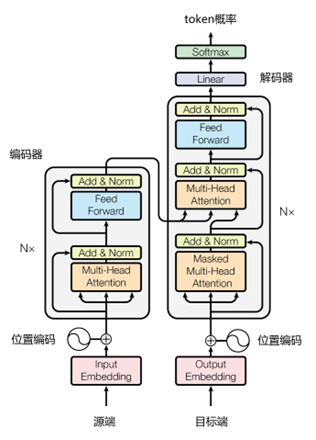
\includegraphics[width=1\textwidth]{figures/Transformer_Structure.png}
	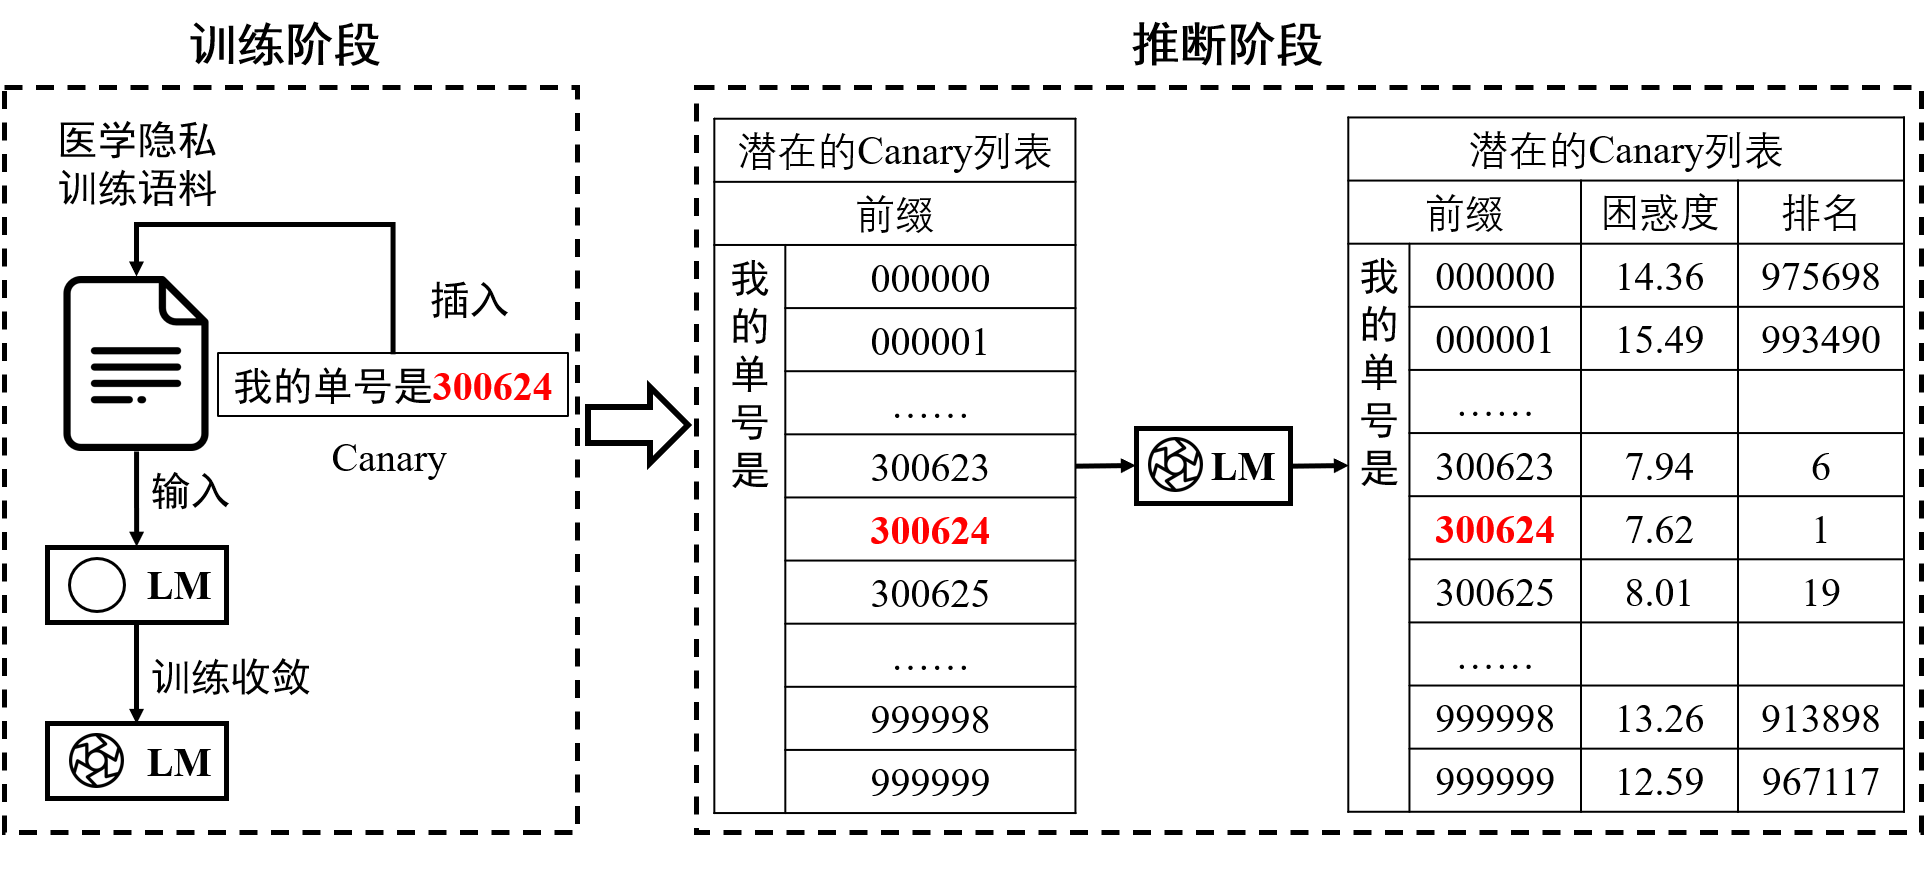
\includegraphics[width=\linewidth]{figures/Chap5_CanaryInsertion.png}
	\caption{Canary插入攻击与衡量}
	\label{Chap5_CanaryInsertion}
\end{figure}


(2)模型反演攻击

%模型反演攻击是针对机器学习模型的一种隐私攻击方法。在这种攻击中,攻击者试图通过已知的模型输出(预测结果)以及对模型的访问权限,推断出输入数据的某些敏感特征。该攻击方法关注的是针对特定个体的信息泄露。
%
%模型反演攻击通常在黑盒和白盒两种情况下进行。在黑盒攻击中,攻击者仅具有有限的模型访问权限,例如仅能使用模型的预测API。攻击者可以通过探测模型的输入-输出关系,以便从模型的预测结果中提取特定用户的敏感信息。黑盒攻击通常需要攻击者具备一定的辅助信息(如输入数据的部分特征或标签信息),以便构建输入并分析输出。在白盒攻击中,攻击者可以直接访问模型的内部结构、权重和参数。这使得攻击者能够更深入地了解模型的工作原理,并更容易地提取输入数据的敏感信息。白盒攻击通常具有更高的成功率,但在实际场景中,攻击者通常很难获得模型的完整访问权限。
%
%模型反演攻击的成因主要是模型在训练过程中学到了输入数据的某些敏感特征。这些特征可能会被用于生成预测结果,从而使攻击者有机会从输出中提取这些特征。

与\ref{训练样本推断攻击-实验设置}节相同,本实验假设恶意攻击者对于模型执行黑盒攻击,即攻击者只能从输入与模型的输出关系来推测隐私信息。

\subsection{实验设置} \label{Chap5_Exp_Setting}

实验环境与\ref{训练样本推断攻击-实验设置}相同,如表\ref{chap4_exp1_env}所示:CPU为AMD Ryzen 9 5900HX、32GB RAM、GPU为RTX3080-Laptop、操作系统为Windows 11 64位。

与\ref{训练样本推断攻击-实验设置}节中的设定相同,本节使用Chinese medical dialogue data (CMDD)中文医疗对话数据集来训练LM。其参数量为81.9M,使用的词表大小为21128,隐层维度为768,12层GPT2Block。与相关工作的设定相同\cite{selectivedp},我们将电话号码、年龄、单号、药物计量、检测的定量结果等数字内容视为敏感信息,并使用正则表达式构建一个策略函数来检测它们。差分隐私中设置$\epsilon=0.5,\delta=\frac{1}{N}=1e-6$(为数据集大小$N$倒数的量级)。本章的实验基于PyTorch的差分隐私库\cite{opacus},以实现相关算法的设计。

为对比本章提出的选择差分隐私的效果,本实验选择两个模型作为对比:
\begin{itemize}
	\item [a)]
	无隐私保护(No\_DP)。这里直接使用原始的训练数据进行训练,可以视为隐私预算$\epsilon=+\infty$。这种情况即为\ref{训练样本推断攻击-实验设置}节中在原始中文预训练模型基础上,利用CMDD数据上微调的模型。
	\item [b)]
	对所有文本进行差分隐私保护(All\_DP)。在这种情况下,把数据集所有的文本当成需要保护的对象。这可以视为选择差分隐私的最坏情况,即$\forall d_i\in D$,策略函数$F$输出$F(d_i)=1$。
	
\end{itemize}

下面介绍上述两种攻击方式的实验设定。

(1)“诱饵”插入攻击

实验中,以"我的单号是 <随机的6位数字>"的形式随机生成了5个Canary:“我的单号是541684”、“我的单号是946241”、“我的单号是197462”、“我的单号是678409”、“我的单号是209118”。每个Canary独立测试,即一个Canary对应一个训练模型。每个实验中,在训练数据集中插入10次Canary(这是一个常见的设定,如\cite{selectivedp}),即在\ref{k_clear_mem}节中定义的10-清晰记忆。

本节以\ref{训练样本推断攻击-实验设置}节中的中文预训练模型为基础,在CMDD数据集上进行微调训练的。分别在64278条训练数据中插入上述Canary 10次,并训练25个epoch,计算在未加保护的情况下,模型的Canary暴露度。


(2)模型反演攻击

与\ref{Chap3_meminfer_setting}节的设定相同,本实验使用随机采样的的10个训练数据的前10个token作为前缀输入,使用\nameref{训练样本推断攻击-实验设置}中的方式分别进行解码,测试其完整恢复训练数据的次数。具体来说,对于每个前缀,本节对上述每个前缀生成10000个解码结果,针对其进行平均统计(平均值为分数则向下取整)。

\subsection{实验结果}

(1)“诱饵”插入攻击

实验中,以"我的单号是 <随机的6位数字>"的形式随机生成了5个Canary:“我的单号是541684”、“我的单号是946241”、“我的单号是197462”、“我的单号是678409”、“我的单号是209118”。每个Canary独立测试,即一个Canary对应一个训练模型。每个实验中,在训练数据集中插入10次Canary(这是一个常见的设定,如\cite{selectivedp}),即在\ref{k_clear_mem}节中定义的10-清晰记忆。

与\ref{chap3_exp_setting}节相同,本节也是以\ref{训练样本推断攻击-实验设置}节中的中文预训练模型为基础,在CMDD数据集上进行微调训练的。分别在64278条训练数据中插入上述Canary 10次,并训练25个epoch,计算在未加保护的情况下,模型的Canary暴露度。

在输入的Canary为“我的单号是541684”时,对没有使用任何隐私保护技术的模型执行攻击,其Canary暴露度如表\ref{Prefix_Attack_Canary}所示。其中,以“‘我的单号是’+ 前缀”表示实际输入模型的完整前缀。

\begin{table}[]
	\centering
	\caption{不同前缀下LM的Canary暴露度}
	\begin{tabular}{|c|c|c|c|c|}
		\hline
		位数&前缀&排名&总可能数&Canary暴露度   \\ \hline
		0&NULL&390111&1e6&1.3588    \\ \hline
		1&5&34986&1e5&1.5152    \\ \hline
		2&54&2597&1e4&1.9451    \\ \hline
		3&541&118&1e3&3.0831   \\ \hline
		4&5416&9&1e2&3.4739    \\ \hline
		5&54168&1&1e1&3.3219    \\ \hline
	\end{tabular}
	\label{Prefix_Attack_Canary}
\end{table}

从表\ref{Prefix_Attack_Canary}可可以看出,在没有隐私保护时,前缀与原训练样本匹配度越高(这里指提供的前缀长度越长),其Canary暴露度越高,即模型越有可能恢复出原始数据,与预期相符。

对于全部5组Canary,其暴露度的平均情况如图\ref{Chap5_DP_Canary_Res}所示,其中No\_DP指在训练与推断阶段均未使用隐私保护技术的模型,All\_DP指对所有训练样本使用DP训练的模型,Seletive\_DP\_Train指对训练样本使用上述实验设置中定义的策略函数的选择差分隐私训练优化器训练的模型,Selective\_DP\_Decode指在训练阶段未使用DP而推断阶段使用选择差分隐私解码算法的模型。

\begin{figure}[h]
	\centering
	%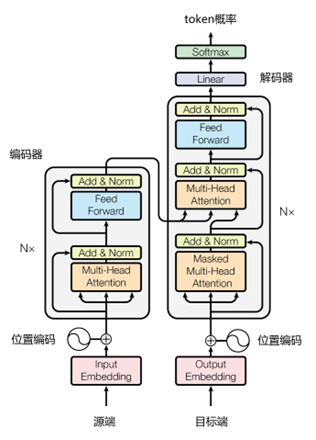
\includegraphics[width=1\textwidth]{figures/Transformer_Structure.png}
	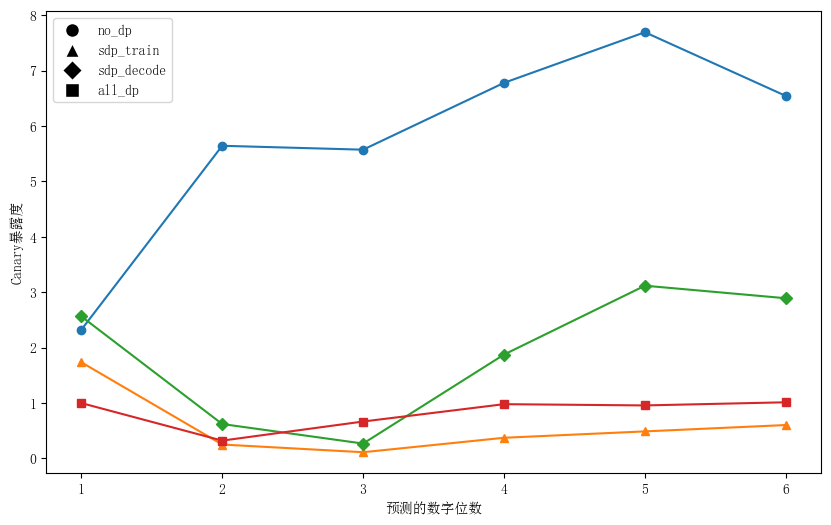
\includegraphics[width=\linewidth]{figures/Chap5_DP_Canary_Res.png}
	\caption{各模型的Canary暴露度}
	\label{Chap5_DP_Canary_Res}
\end{figure}

可以从图\ref{Chap5_DP_Canary_Res}看出,No\_DP的Canary暴露度最高,而All\_DP的Canary暴露度最少;Seletive\_DP\_Train与Seletive\_DP\_Decode表现效果相似,介于All\_DP与No\_DP之间且表现效果更接近All\_DP。因此可以证明Seletive\_DP\_Train与Seletive\_DP\_Decode均对训练数据的隐私起到了保护作用,保护程度都接近与All\_DP的效果。

表\ref{Chap5_Mode_PPL},表示No\_DP、All\_DP、Seletive\_DP\_Train与Seletive\_DP\_Decode的困惑度指标。由定义\ref{PPL}可知,困惑度是描述模型对于测试样本语句整体的“惊讶”程度,若模型效果好,那么测试的文本对模型而言就很正常,困惑度就不会很高,反之亦然。

\begin{table}[]
	\centering
	\caption{不同方式下的模型困惑度}
	\begin{tabular}{|c|c|}
		\hline
		方式&困惑度   \\ \hline
		No\_DP&11.22    \\ \hline
		All\_DP&59.75    \\ \hline
		Seletive\_DP\_Train&21.32    \\ \hline
		Seletive\_DP\_Decode&13.58   \\ \hline
	\end{tabular}
	\label{Chap5_Mode_PPL}
\end{table}

表\ref{Chap5_Mode_PPL}中不同情况差别很大。这主要是与PPL的计算方式有关。PPL可以视为模型对测试数据集中每句话的交叉熵Loss的指数结果的均值,即$PPL(D)=\frac{1}{N}\sum_{i=1}^{N}\exp(Loss(Model(S_i)))$,其中$D=\{S_1,S_2,\cdots, S_N\}$。在CMDD数据集上训练的Loss在2-4之间,由交叉熵的定义可知,模型平均Loss为2即相当于在$e^2=7.389$个Token中随机猜测,而Loss为2即相当于在$e^4=54.598$个Token中随机猜测,相比与词表大小13317,该预测结果较好。那么在这种情况下的PPL的变化就会从$e^2=7.389$到$e^4=54.598$,因此上述PPL的范围也符合预期。

从上述结果可以看出,No\_DP的PPL最低,即模型对测试数据不“惊讶”,意味着该模型生成效果最好,而All\_DP的效果最差,是因为它将所有文本视为隐私信息,而忽略了大部分内容是不敏感的。有趣的是虽然前面Seletive\_DP\_Train与Seletive\_DP\_Decode的Canary暴露度相近,而Seletive\_DP\_Decode的PPL要比Seletive\_DP\_Train低了36\%,这是由于Seletive\_DP\_Decode的训练过程是正常的,只是在推断阶段在生成的隐私内容上加噪,而Seletive\_DP\_Train虽然只是对隐私部分的内容加噪,但是其在隐私内容的语义范式上加噪会降低模型的表达能力。另一方面,由于上面PPL差异大的分析,回到平均Loss的空间下,二者分别为2.609与3.059,这在图\ref{Chap3_train_loss}所示的训练情况下差别并不大。

(2)模型反演攻击



表\ref{Chap5_Mem_Infer_Number},表示No\_DP、All\_DP、Seletive\_DP\_Train与Seletive\_DP\_Decode情况下的成员推断成功次数。从中可以看出使用All\_DP取得了10000个生成样本中没有任何成功恢复的效果,而Seletive\_DP\_Train和Seletive\_DP\_Decode仅比No\_DP的成功次数少一点,与All\_DP之间的差别还是很大。

\begin{table}[]
	\centering
	\caption{攻击方式与成功次数}
	\begin{tabular}{|c|c|}
		\hline
		类型&成功次数   \\ \hline
		No\_DP& 14    \\ \hline
		All\_DP& 0   \\ \hline
		Seletive\_DP\_Train&13    \\ \hline
		Seletive\_DP\_Decode&11    \\ \hline
	\end{tabular}
	\label{Chap5_Mem_Infer_Number}
\end{table}

产生这种现象的也是符合逻辑与预期的,主要原因如下:

\begin{itemize}
	\item [a)]
	由于在\ref{Chap5_Exp_Setting}节的设定下,策略函数仅将数字部分当作隐私内容,对其使用相应的DP方法处理,非数字内容占比很大,导致模型更容易记忆住这些非数字内容。因此,虽然Seletive\_DP\_Train与Seletive\_DP\_Decode采用相应的符合选择差分隐私定义的步骤进行处理,但是保护的内容较少,成员推断攻击只关注于某句子是否在训练语料中出现,所以这两者的保护效果相对于No\_DP差别很小。相反,All\_DP对所有的样本都执行了差分隐私处理,因此面对成员推断攻击这种需要对样本整体内容验证的方法保护效果较好。
	\item [b)]
	CMDD的训练语料相对于预训练模型的语料较少,在微调的过程中,由于预训练语料的分布差别很大的医学文本语料具有特殊性,在多轮训练后模型会逐渐记住这种风格类型于具体的数据内容,因此在数据量较少的数据集上微调会让模型更容易记住该数据集。
	
\end{itemize}

%\subsection{实验分析}
%
%从攻击结果来看,攻击提供的前缀位数越多,模型的Canary暴露度越高,即模型越有可能恢复出原始的训练文本。
为防止攻击者在推断阶段试图通过执行输入和标签重构攻击,以恢复训练隐私数据,同时保持语言模型的表现效果,本章提出了一个基于差分隐私的新颖的隐私保护算法——选择差分隐私算法。首先,本章将介绍系统模型与设计目标,引入本章的保护对象与攻击者的行为。其次,介绍选择差分隐私的定义,并针对训练与推断阶段分别设计了隐私优化器与解码算法,作为两种提供选择差分隐私的方式。随后,对前述设计的隐私优化器与解码算法进行隐私性分析,以证明其满足差分隐私的定义。最后,通过设计实验说明选择差分隐私以及这两种保护方式的优势。


\section{本章小结}

本章首先对该场景下的系统模型与设计目标进行介绍,随后引入了选择差分隐私的概念,并针对并针对训练与推断阶段分别设计了隐私优化器与解码算法,作为两种提供选择差分隐私的方式。在理论分析完这两种方式的安全性后,通过基于预训练模型在CMDD数据集上微调的实验,将各种设定下的结果进行对比分析,证明了本章提出的选择差分隐私的优势。